The two friends set off on the skateboard with Charlie in front and Emily close at the back, holding onto Charlie as to not fall off of the vehicle.

Occasional gusts of wind hit their faces as they passed beautiful lanes filled with stores.

Emily, being as excited as she was about her date with Matthew, became more and more worried about her best friend as they passed his favorite shop, "Skate 4 life", with all the very cool skateboards displayed in the window, and he didn't even stop to press his nose against the glass and stare at them.

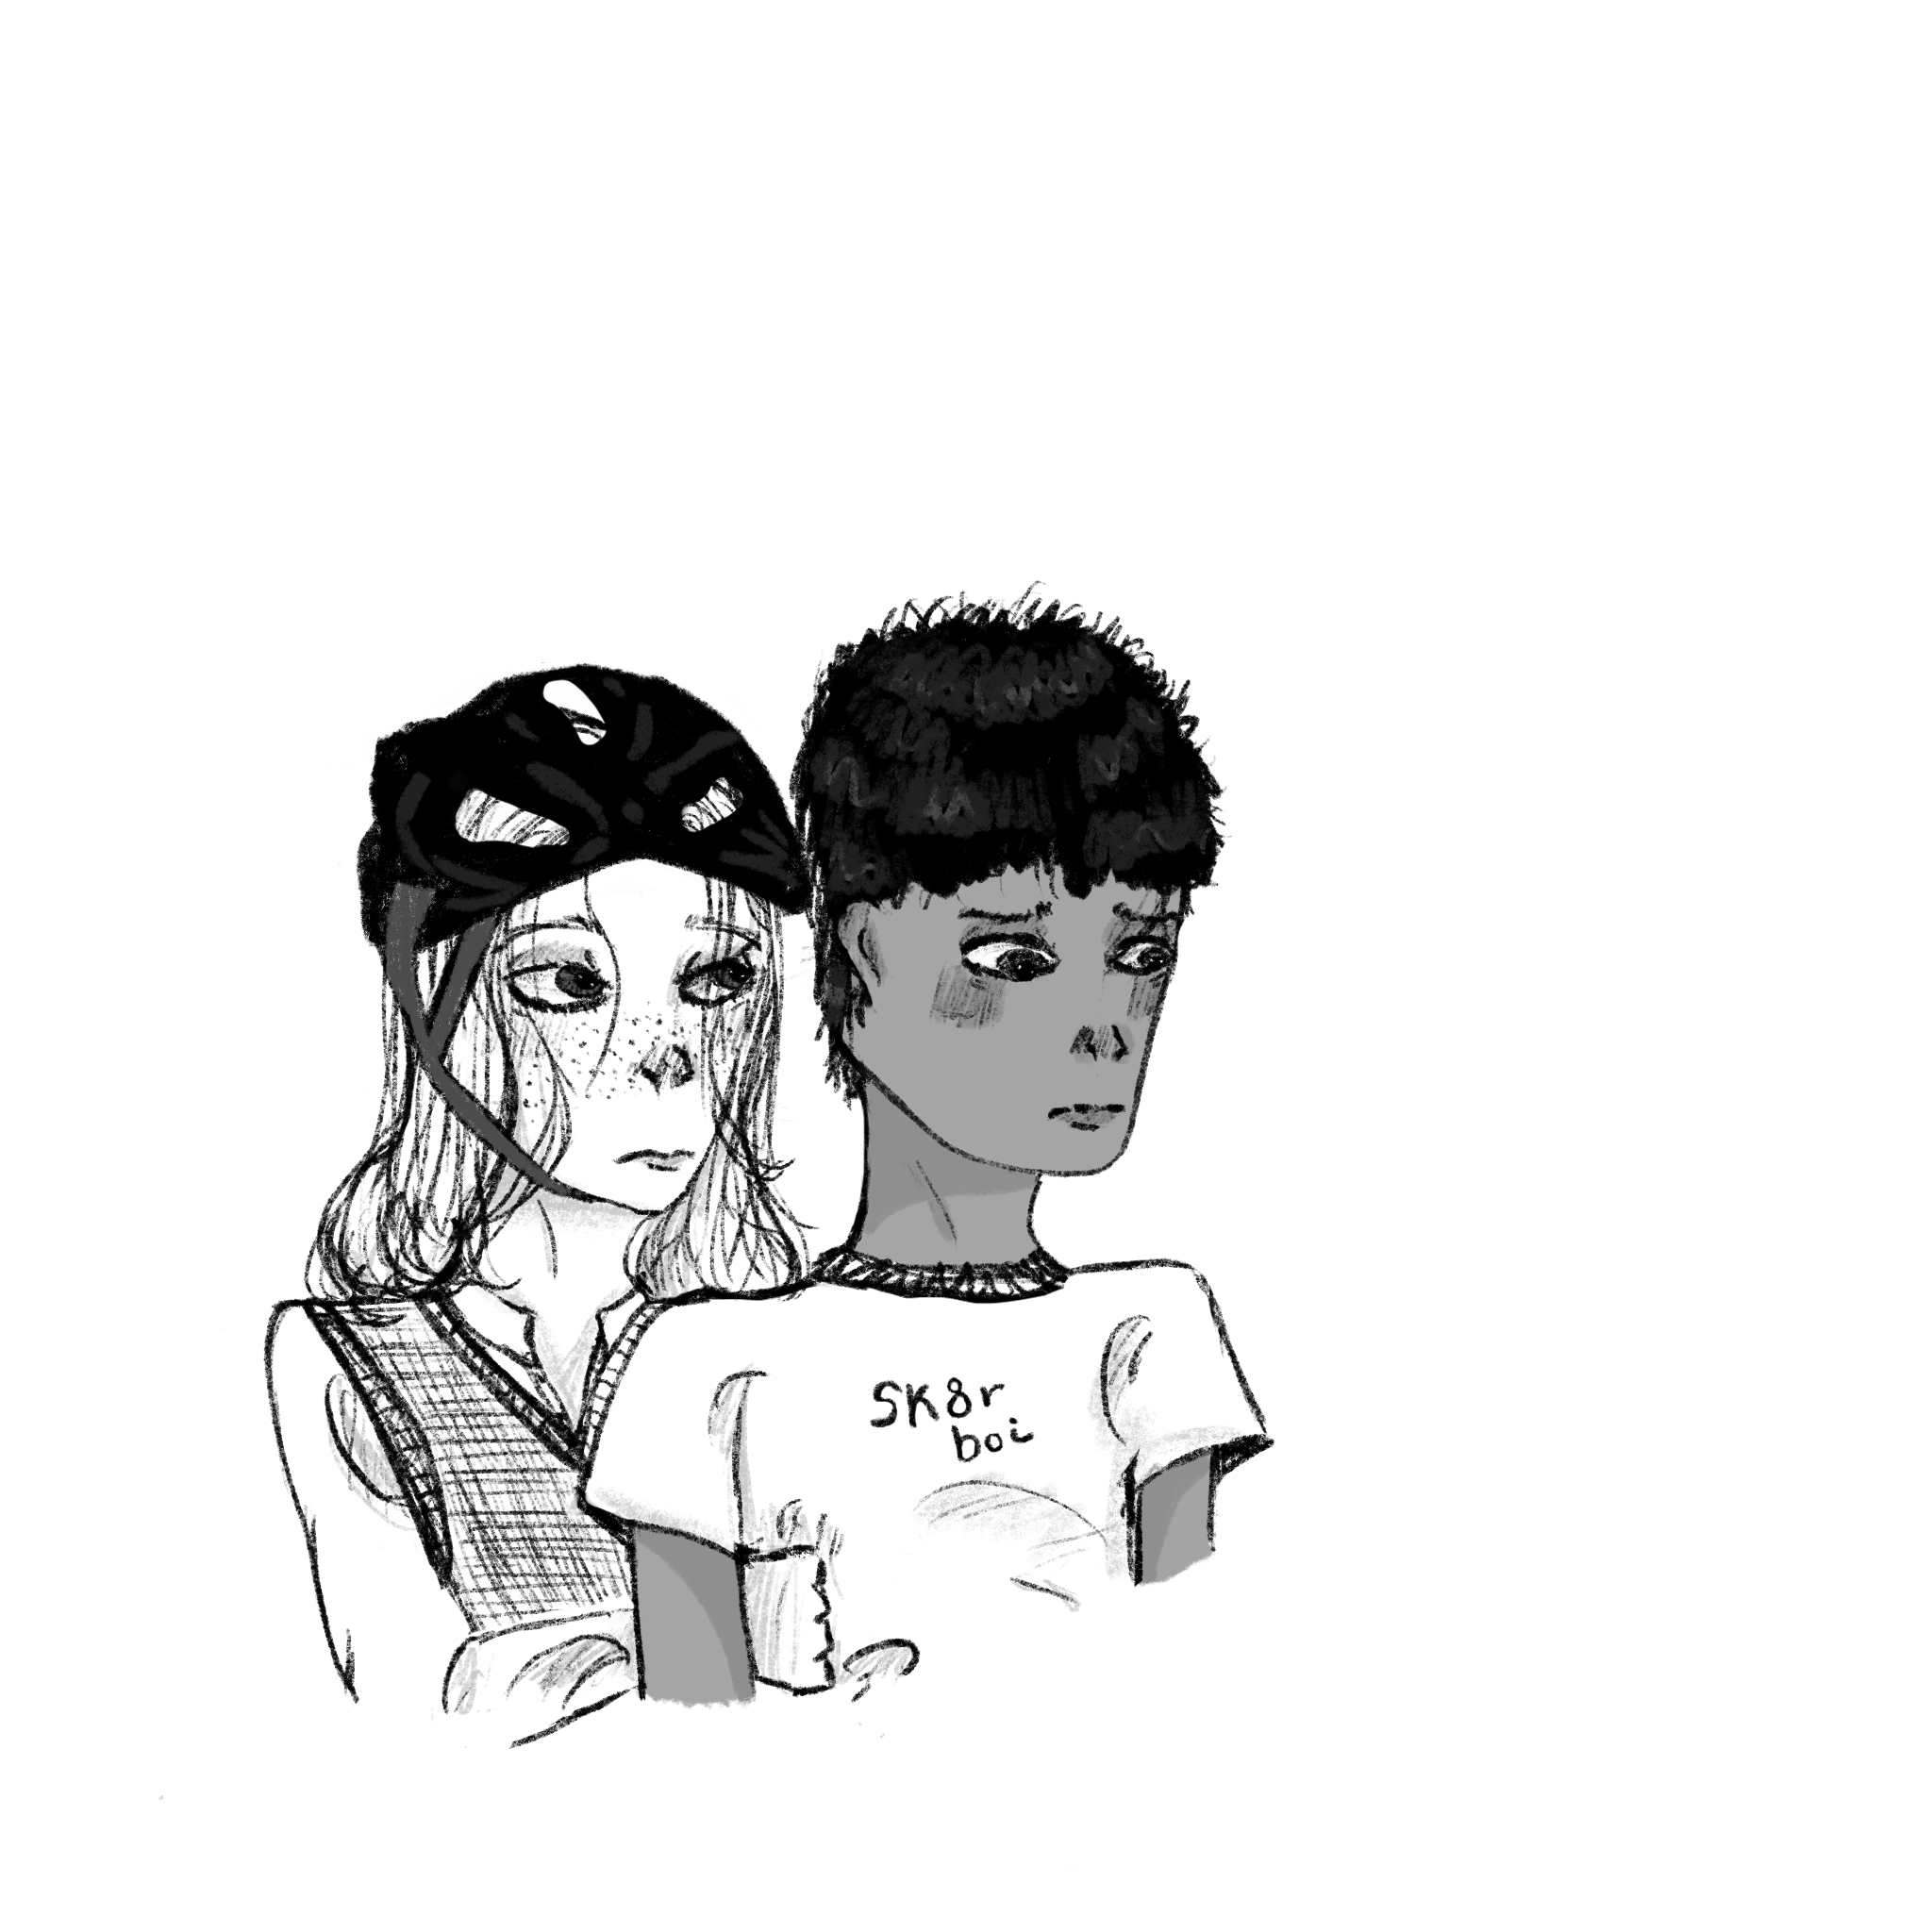
\includegraphics[width=0.99\textwidth]{Emily&Charlie.png}

The most worrisome fact was that Charlie didn't put on any helmet at all, which was so peculiar, seeing as he was crazy about safety and never rode around on his skateboard without it.

The whole journey to the frozen yogurt store was quiet and sad. Charlie's expression of grief deepened as they caught the last blast of wind, their clothes—Emily's white blouse and Charlie's T-shirt with "Sk8r Boi" embroidered on it—fluttering for the last time before the friends stopped in front of the pastel-pink building. The grounds were decorated with rose bushes serving as a fence and a neat stone path leading up to a glass door with an "Open" sign on it.

“Charlie, are you alright?” Emily asked as she got off and handed him his helmet.

“Yes. Yes, I am,” Charlie answered as he put his helmet back on, but stopped mid-action, “In fact, I'm better than 'alright'. You know, I don't actually need this helmet anymore… so you can keep it. I mean, if Miller doesn't wear one, then why do \textit{I} need to?”

He gave his helmet back to Emily, looking anxiously at it. She looked apprehensively at him.

“But what do I do with it…?” Emily started.

“It's okay. I don't need it,” Charlie interrupted her.

“Well, I better go then…” The blond girl turned to face the building and started walking up the way.

“But don't expect me to wait for you and give you a ride home after!” Charlie yelled, ready to set off. “I have other plans… with my friends, who are skaters, like me…!”

“Don't worry about it,” Emily replied sweetly as she entered the building.

Inside was even nicer than the outside with about a dozen cute sky-blue circular tables and about three times more stools of the same kind. There was a counter with four cash registers, a menu above them and a door to the right of the counter which assumingly led to the kitchen.

Most of the tables were occupied and one of the occupants was, in fact, Matthew Miller, sitting at one of the tables all alone. Emily took a deep breath and walked up to him. As he noticed her, he immediately stood up and greeted her with a smile. Emily returned his smile with a nervous one of her own. And the date began.